\def\x{x}
\def\Q{Q}
\def\bds#1{#1}

\section{Experiments}
\label{sec:thesims}
%\subsection{Simulations}
We first illustrate our methods using a simulation of the model
\begin{equation}\nonumber
         Y_i = \x_{iS}^{\top}\Q\x_{iS} + \epsilon_i \quad (i=1,2,\ldots,n).
\end{equation}
Here $\x_{i}$ denotes data sample $i$ drawn from $\mathcal{N}(\bds{0},\bds{I}_{p})$, 
$\x_{iS}$ is a subset of $\x_i$ with dimension $|S|=5$, where $S$
represents the relevant variable set, and 
$\epsilon_i$ is additive noise drawn from $\mathcal{N}(0,1)$. 
The matrix $\Q$ is a symmetric positive definite matrix of dimension $|S|\times{}|S|$. 
Note that if $\Q$ is diagonal, then the true function is convex
additive; 
otherwise the true function is convex but not additive.
For all simulations in this section, we set $\lambda=4\sqrt{{\log(np)}/{n}}$.

In the first simulation, we set $\Q=\bds{I}_{|S|}$ (the additive
case), and choose $n=100, 200,\ldots,1000$ and $p=64,128,256,512$.
For each $(n,p)$ combination, we generate $200$ independent data
sets. For each data set we use SCAM to infer the model parameterized
by $\bds{h}$ and $\bds{\beta}$; see equation \eqref{np}. If
$\|\bds{\beta}_{k\cdot}\|_{\infty}<10^{-8}\ (\forall k\not\in{}S)$ and
$\|\bds{\beta}_{k\cdot}\|_{\infty}>10^{-8}\ (\forall k\in{}S)$, then
we declare correct support recovery. We then plot the probability of
support recovery over the $200$ data sets in Figure \ref{Support}(a).  We
observe that SCAM performs consistent variable selection when the true
function is convex additive.  
To give the reader a
sense of the running speed, the code runs in about $2$ minutes on one
data set with $n=1000$ and $p=512$, on a MacBook with 2.3 GHz Intel
Core i5 CPU and 4 GB memory.

In the second simulation, we study the case in which the true function
is convex but not additive. We generate four $\Q$ matrices
plotted in Figure \ref{Support}(b), where the diagonal elements are all $1$ and
the off-diagonal elements are $0.5$ with probability $\alpha$
($\alpha=0,0.2,0.5,1$ for the four cases). We fix $p=128$ and choose
$n=100,200,\ldots,1000$. We again run the SCAM optimization on $200$
independently generated data sets and plot the probability of recovery
in Figure \ref{Support}(c). The results demonstrate that SCAM performs
consistent variable selection even if the true function is not additive (but
still convex).

In the third simulation, we study the case of correlated design, where
$\x_{i}$ is drawn from $\mathcal{N}(\bds{0},\bds{\Sigma})$
instead of $\mathcal{N}(\bds{0},\bds{I}_{p})$, with
$\Sigma_{ij}=\nu^{|i-j|}$. We use the non-additive $\Q$ with
$\alpha=0.5$ and fix $p=128$.  The recovery curves for $\nu=02, 0.4,
0.6, 0.8$ are depicted in Figure \ref{Support}(d). As can be seen, for
design of moderate correlation, SCAM can still select relevant
variables well.


%\begin{figure}[!htpb]
%        \centering
%        \begin{subfigure}[b]{0.45\textwidth}
%                \centering
%                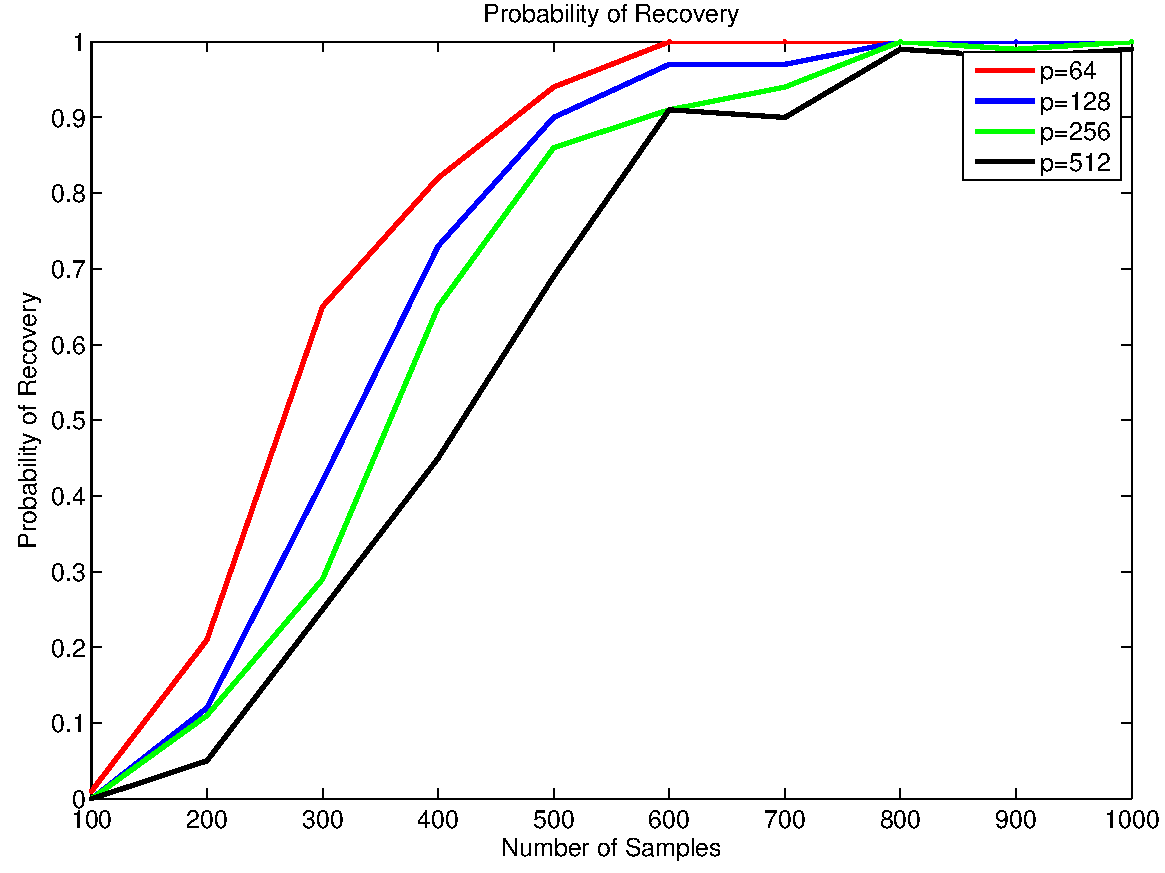
\includegraphics[width=\textwidth]{figs/Curve1}
%                 \caption{Additive model.}
%                \label{Curve1}
%        \end{subfigure}
%        \begin{subfigure}[b]{0.45\textwidth}
%                \centering
%                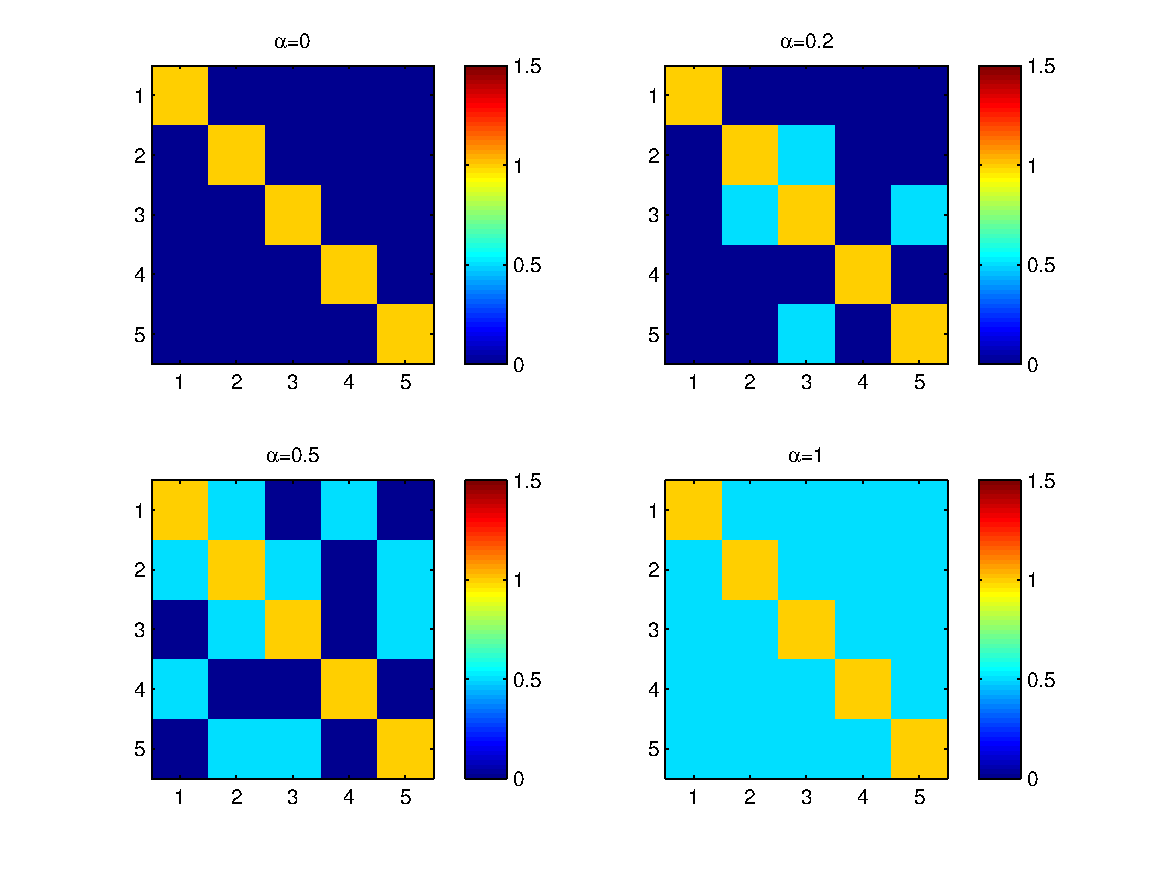
\includegraphics[width=\textwidth]{figs/Q}
%                \caption{Four $\Q$ matrices.}
%                \label{Q}
%        \end{subfigure}\\
%        \begin{subfigure}[b]{0.45\textwidth}
%                \centering
%                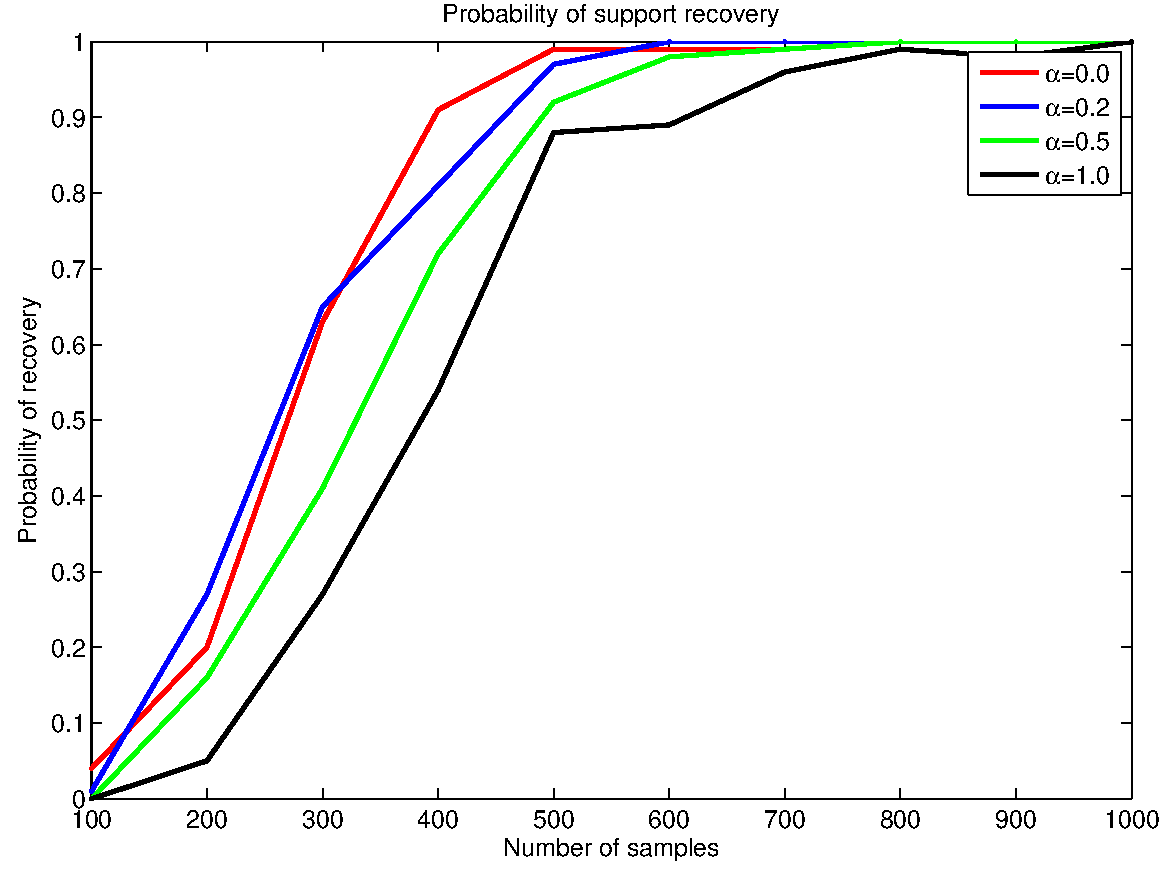
\includegraphics[width=\textwidth]{figs/Curve2}
%                \caption{Additive and non-additive models.}
%                \label{Curve2}
%        \end{subfigure}
%        \begin{subfigure}[b]{0.45\textwidth}
%                \centering
%                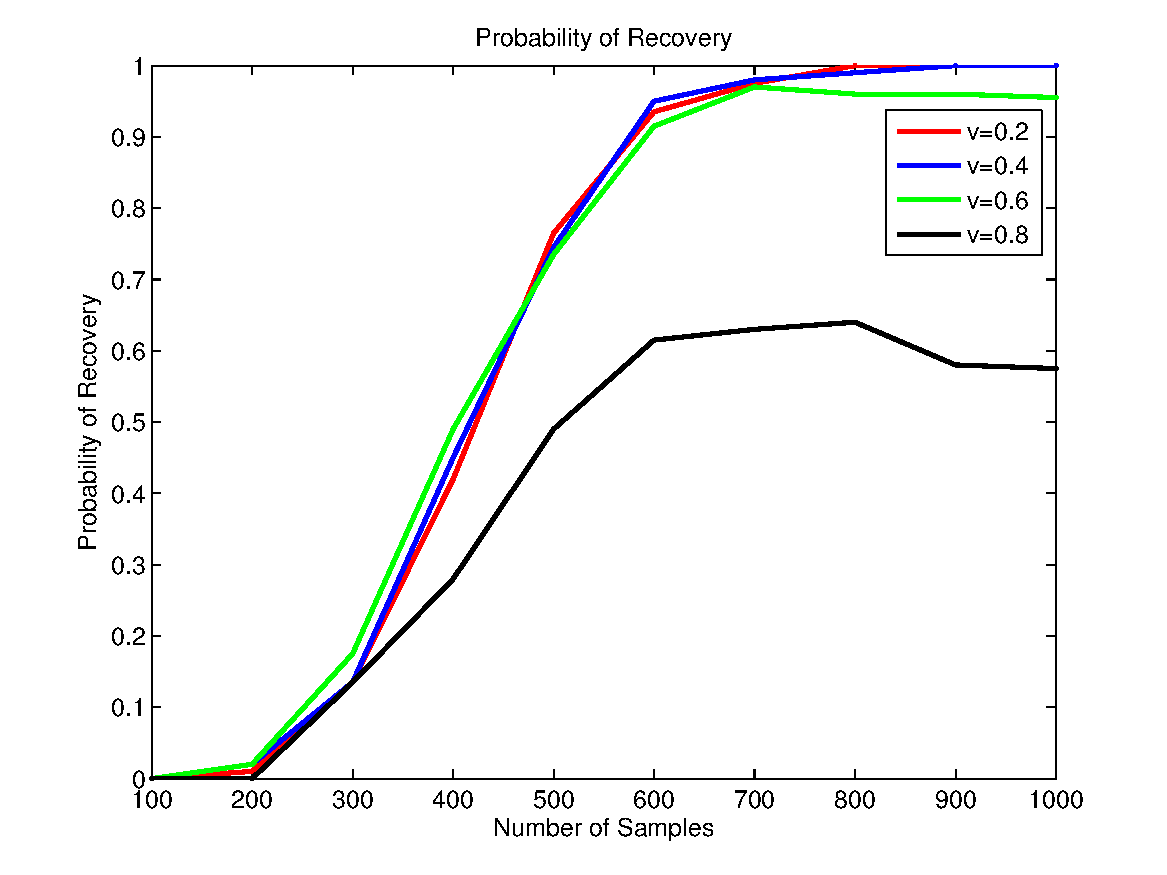
\includegraphics[width=\textwidth]{figs/Curve3}
%                \caption{Correlated design for non-additive model.}
%                \label{Curve3}
%        \end{subfigure}
%        \caption{Result of support recovery.}\label{Support}
%\end{figure}

%\begin{figure}[ht]
%\begin{center}
%\begin{tabular}{cccc}
%\hskip-20pt
%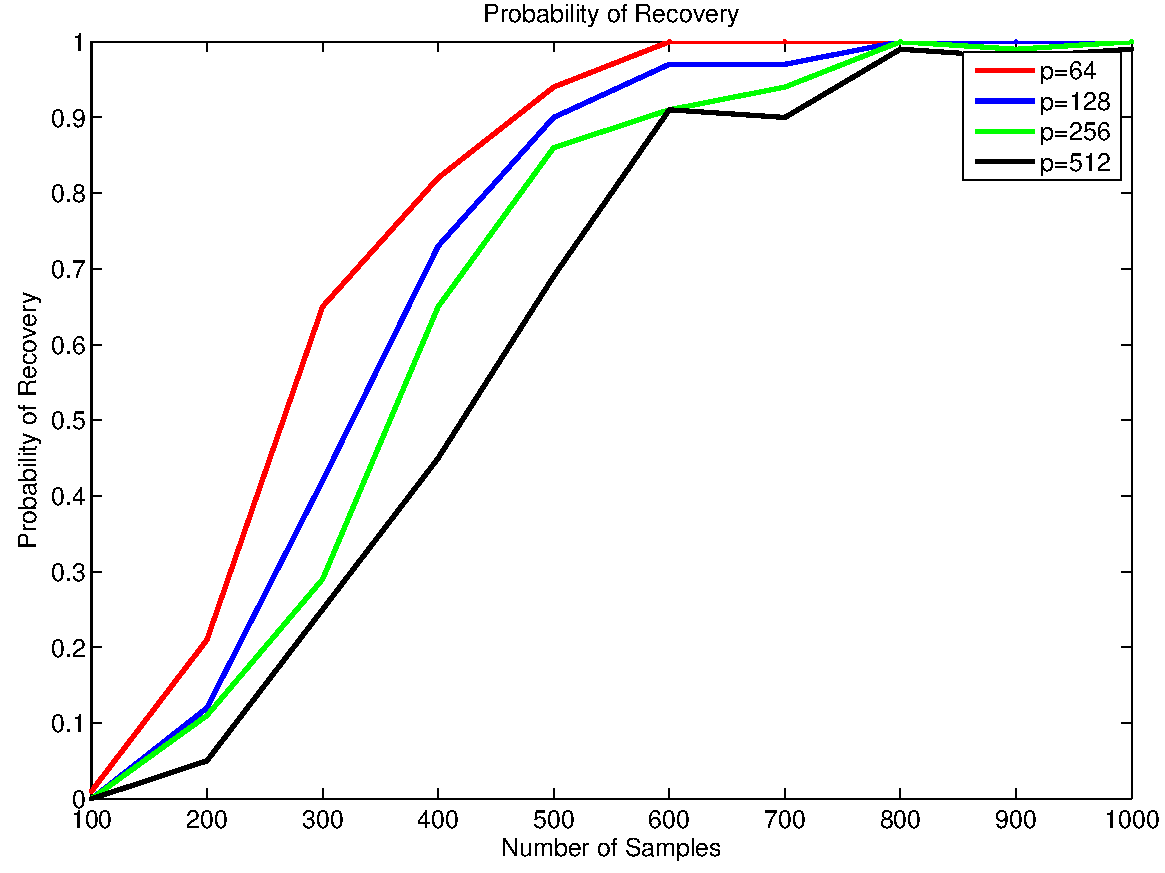
\includegraphics[width=.27\textwidth]{figs/Curve1} &
%\hskip-17pt
%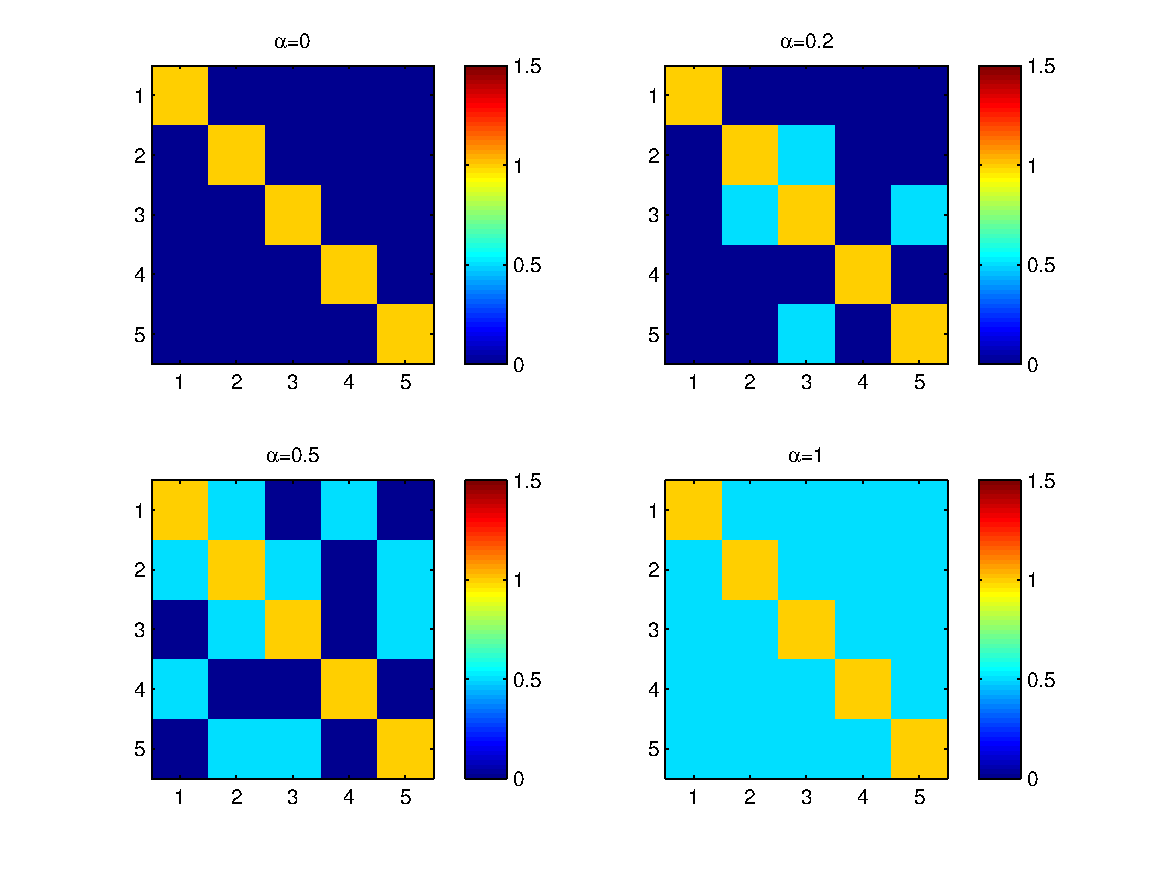
\includegraphics[width=.27\textwidth]{figs/Q} &
%\hskip-17pt
%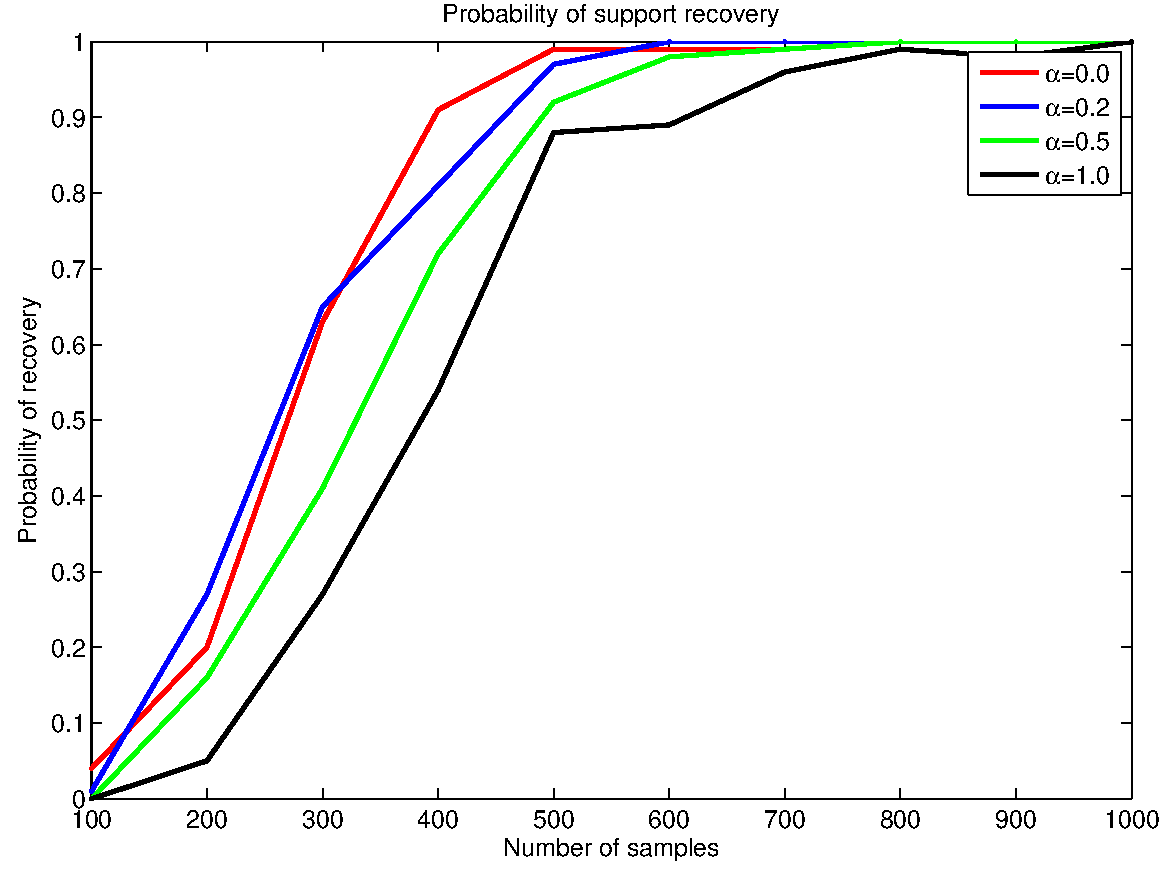
\includegraphics[width=.27\textwidth]{figs/Curve2} &
%\hskip-17pt
%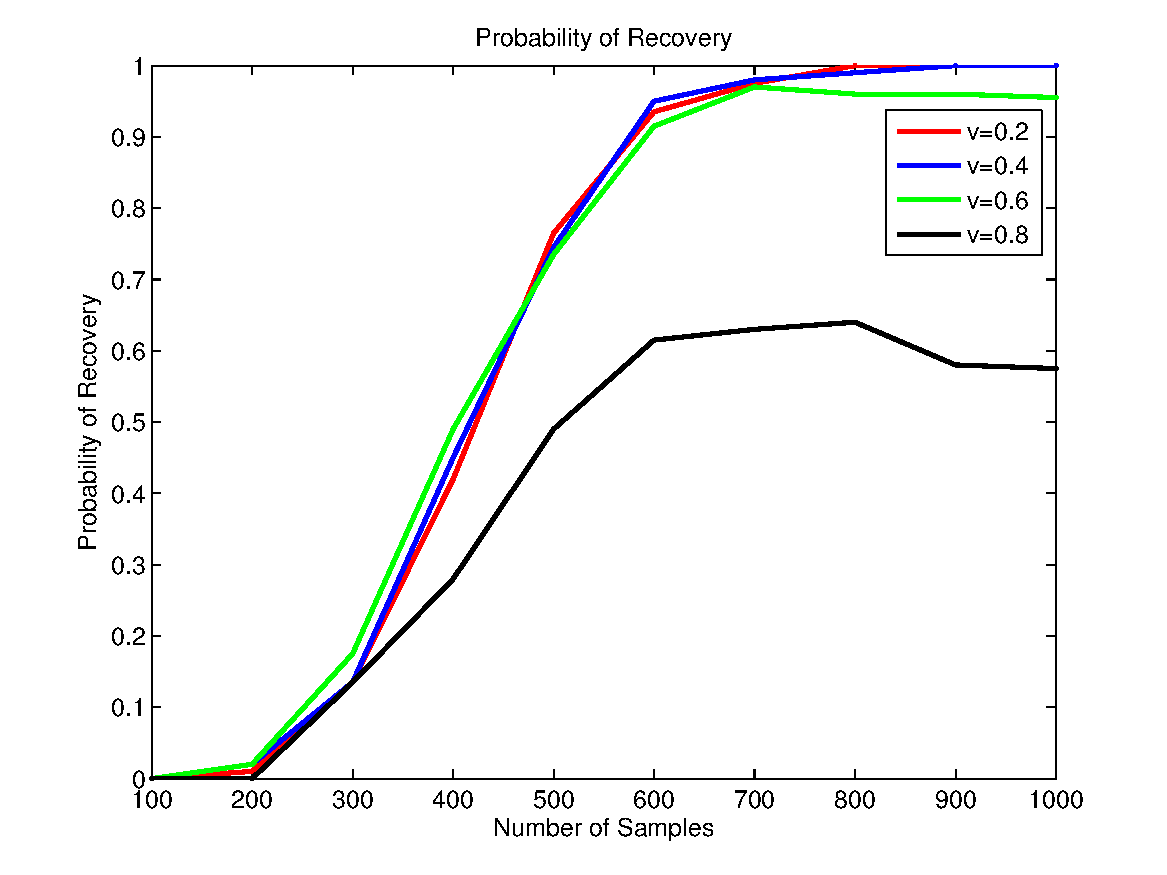
\includegraphics[width=.27\textwidth]{figs/Curve3}  \\
%(a) additive model & (b) four $\Q$ matrices &
%(c) non-additive models & (d) correlated design
%\end{tabular}
%\end{center}
%\caption{Result of support recovery.}\label{Support}
%\end{figure}


%\subsection{Boston housing data}

We next use the Boston housing data rather than simulated data. This data set
contains 13 covariates, 506 samples and one response variable
indicating housing values in suburbs of Boston. The data and detailed description
can be found on the UCI Machine Learning Repository website~\footnote{\texttt{http://archive.ics.uci.edu/ml/datasets/Housing}}. 

We first use all $n=506$ samples (with normalization) to train SCAM, using
a set of candidate $\{\lambda^{(t)}\}$ with $\lambda^{(1)}=0$ (no regularization). For each $\lambda^{(t)}$
we obtain a subgradient matrix $\bds{\beta}^{(t)}$ with $p=13$ rows. The non-zero
rows in this matrix indicate the variables selected using $\lambda^{(t)}$. 
We plot $\|\bds{\beta}^{(t)}\|_{\infty}$ and the row-wise mean of $\bds{\beta}^{(t)}$ versus the normalized
norm $\frac{\|\bds{\beta}^{(t)}\|_{\infty,1}}{\|\bds{\beta}^{(1)}\|_{\infty,1}}$ in Figures \ref{Boston}(a) and \ref{Boston}(b).
As a comparison we plot the LASSO/LARS result in a similar way in Figure \ref{Boston}(c).
From the figures we observe that the first three variables selected by SCAM
and LASSO are the same: LSTAT, RM and PTRATIO, which is consistent with previous findings~\cite{SpAM:07}.
The fourth variable selected by SCAM is TAX (with $\lambda^{(t)}=0.09$).
We then refit SCAM with only these four variables without regularization, and plot the inferred additive
functions in Figure \ref{Boston}(e). As can be seen, these functions contain clear nonlinear effects which cannot be captured
by LASSO. The shapes of these functions are in agreement with those obtained by SpAM~\cite{SpAM:07}.

Next, in order to quantitatively study the predictive performance, we run 10 times 5-fold cross validation, following
the same procedure described above (training, variable selection and
refitting).  A plot of the mean and standard
deviation of the predictive Mean Squared Error (MSE) in in Figure \ref{Boston}(d). Since for SCAM the same $\lambda^{(t)}$ may lead to
slightly different number of selected features in different folds and runs, the values on the x-axis (average number of selected features)
for SCAM are not necessarily integers. Nevertheless, the figure clearly shows that SCAM has a much lower predictive MSE than LASSO. 
We also compared the performance of SCAM with that of Additive Forward Regression (AFR) presented in~\cite{Xi:09}, and found that they are similar.
The main advantages of SCAM compared with AFR and SpAM are 1) there are no other tuning parameters (such as bandwidth)
besides $\lambda$; 2) SCAM is formulated as a convex program, which guarantees a global optimum.

%\begin{figure}[!htpb]
%        \centering
%        \begin{subfigure}[b]{0.45\textwidth}
%                \centering
%                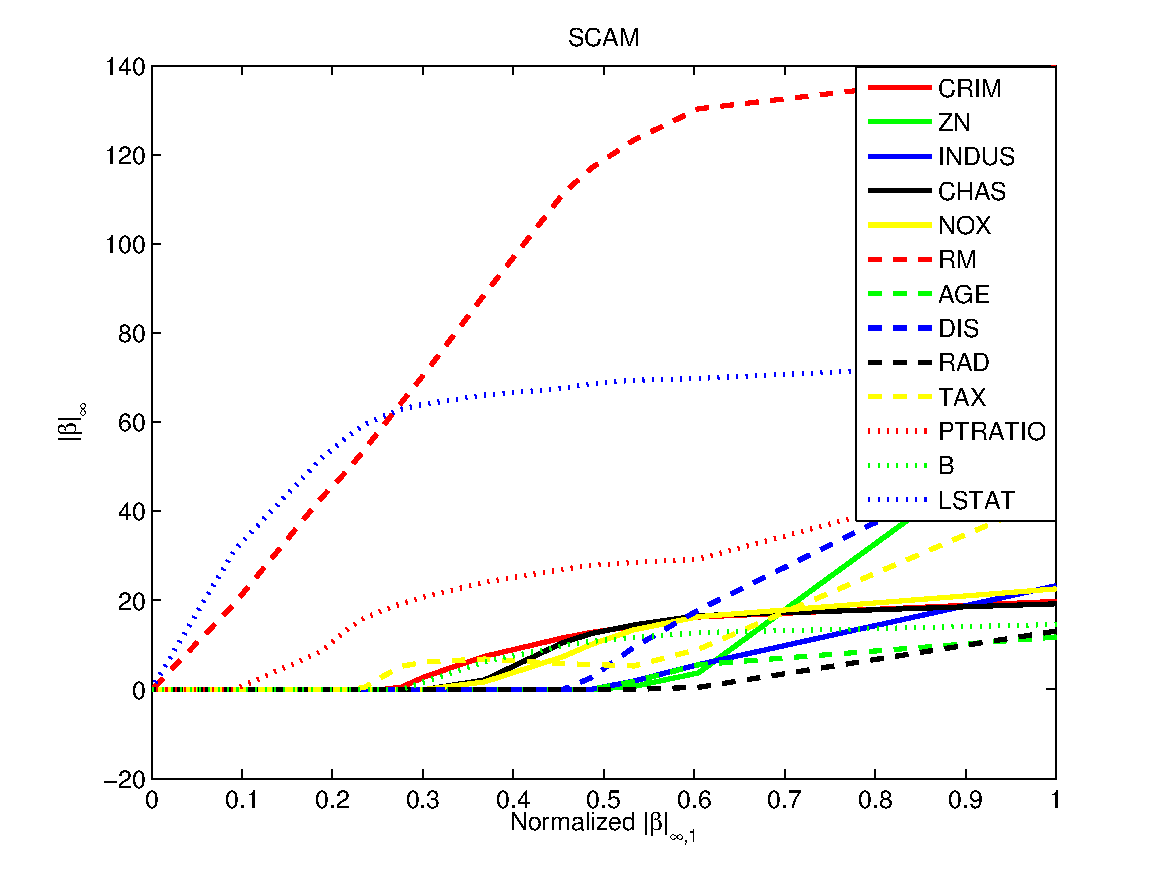
\includegraphics[width=\textwidth]{figs/Additive}
%                 \caption{Variable selection result using SCAM.}
%                \label{SCAM}
%        \end{subfigure}
%        \begin{subfigure}[b]{0.45\textwidth}
%                \centering
%                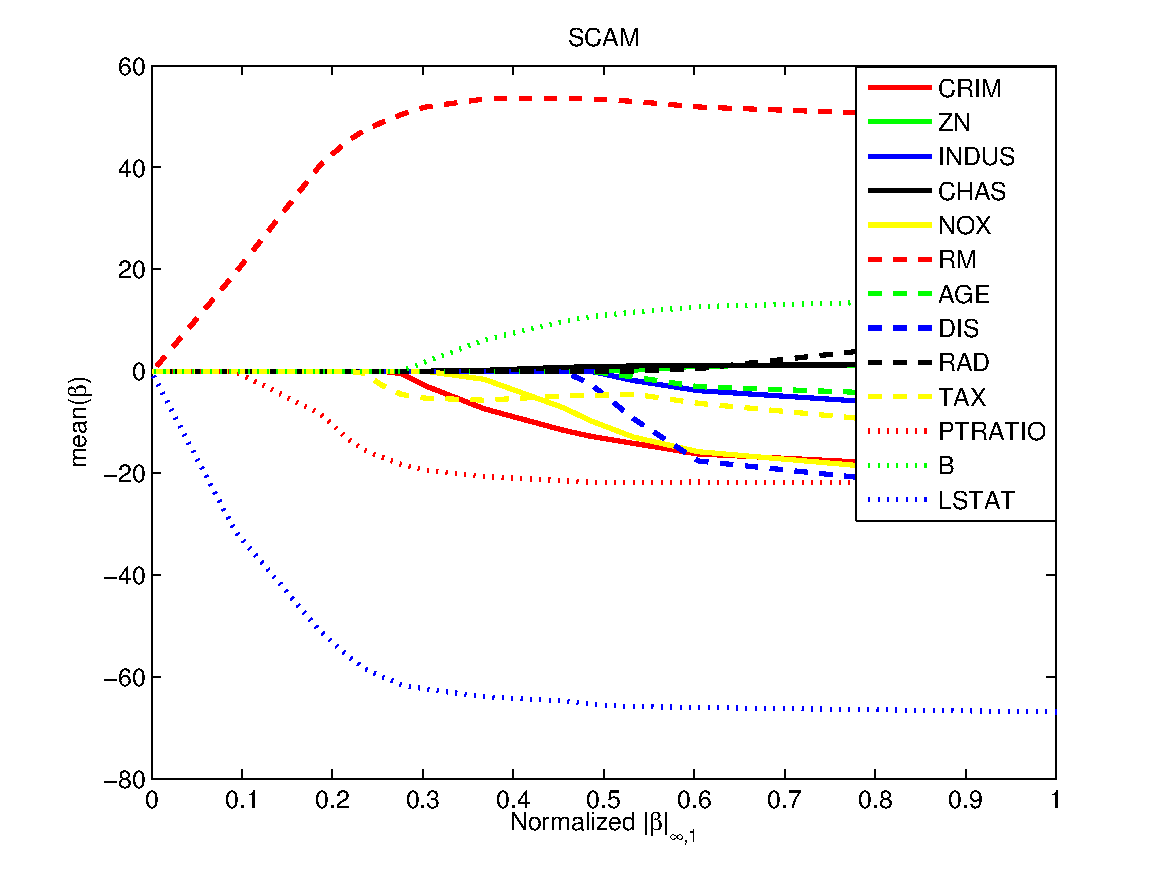
\includegraphics[width=\textwidth]{figs/Additive1}
%                 \caption{Variable selection result using SCAM.}
%                \label{SCAM1}
%        \end{subfigure}\\
%        \begin{subfigure}[b]{0.45\textwidth}
%                \centering
%                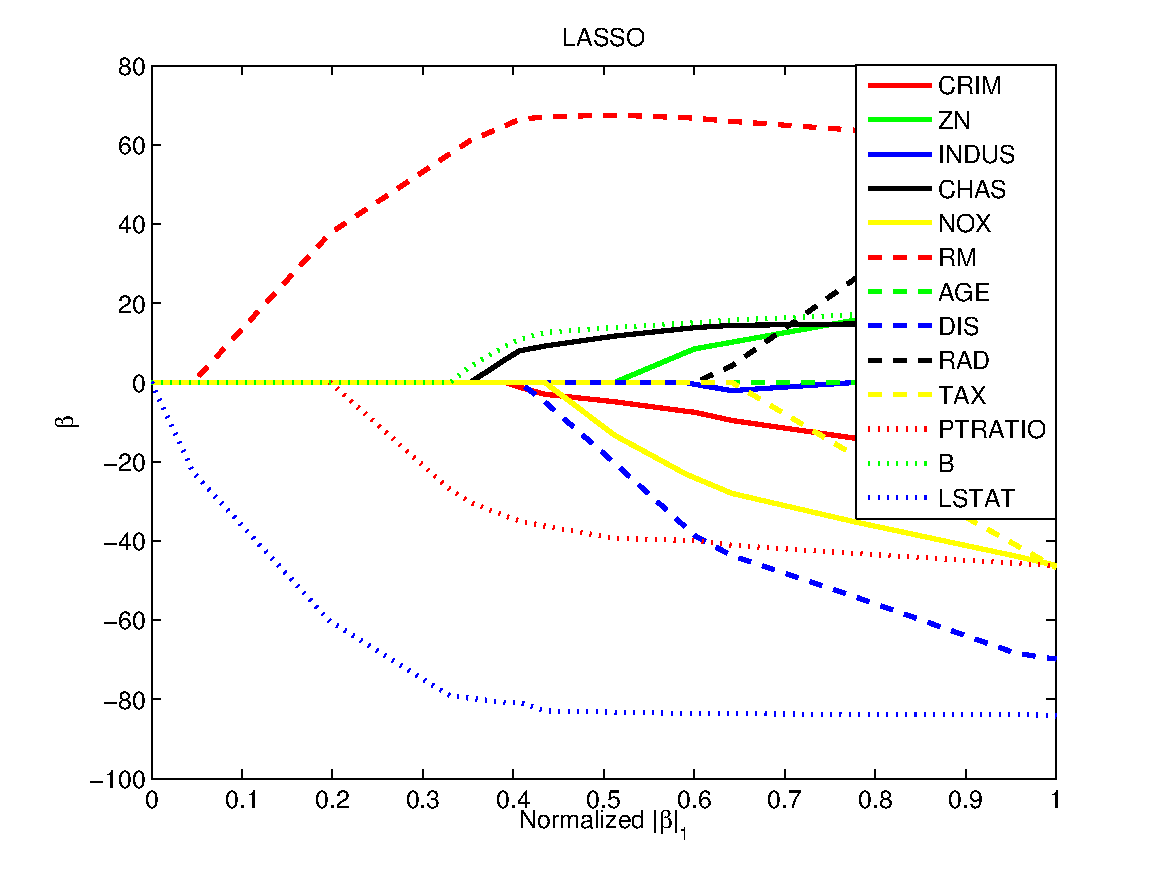
\includegraphics[width=\textwidth]{figs/LASSO}
%                \caption{Variable selection result using LASSO.}
%                \label{LASSO}
%        \end{subfigure}
%        \begin{subfigure}[b]{0.45\textwidth}
%                \centering
%                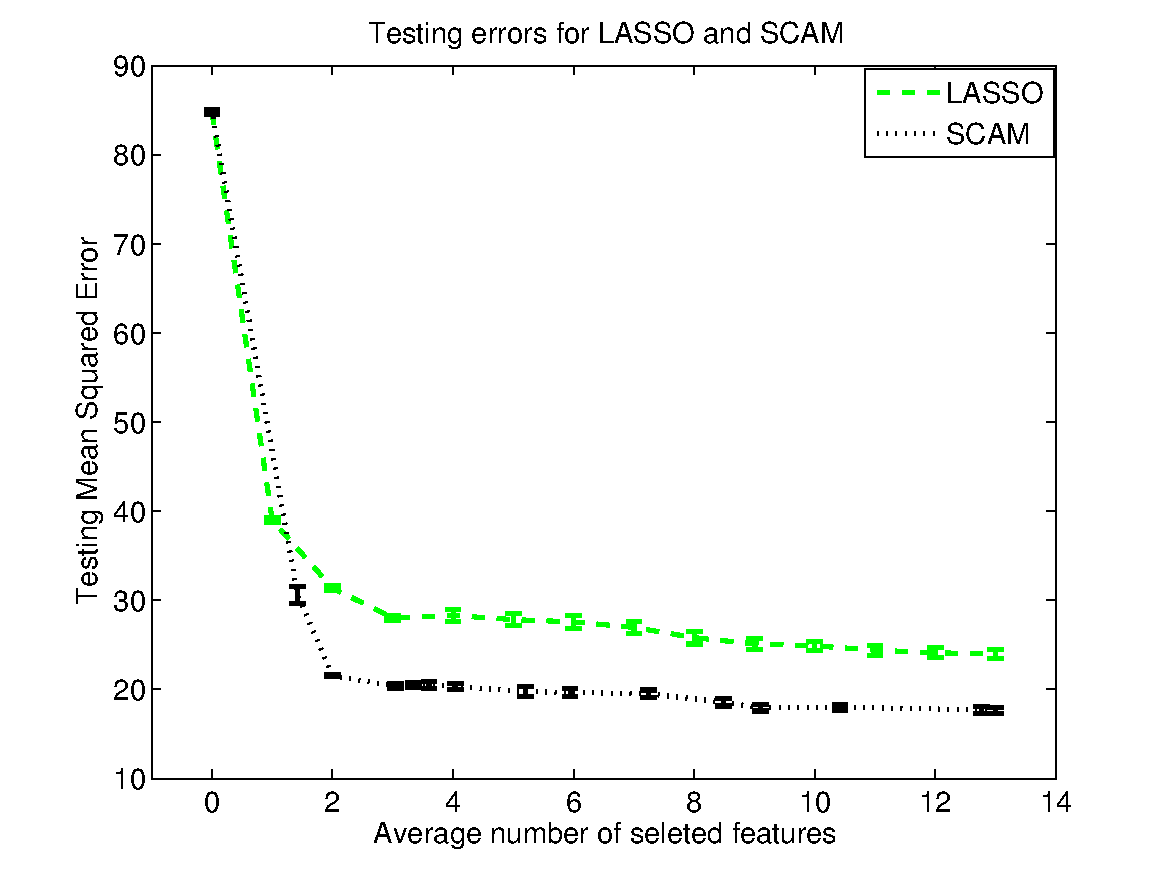
\includegraphics[width=\textwidth]{figs/MSE}
%                 \caption{Predictive MSE of SCAM and LASSO.}
%                 \label{MSE}
%        \end{subfigure}\\
%        \begin{subfigure}[b]{0.45\textwidth}
%                \centering
%                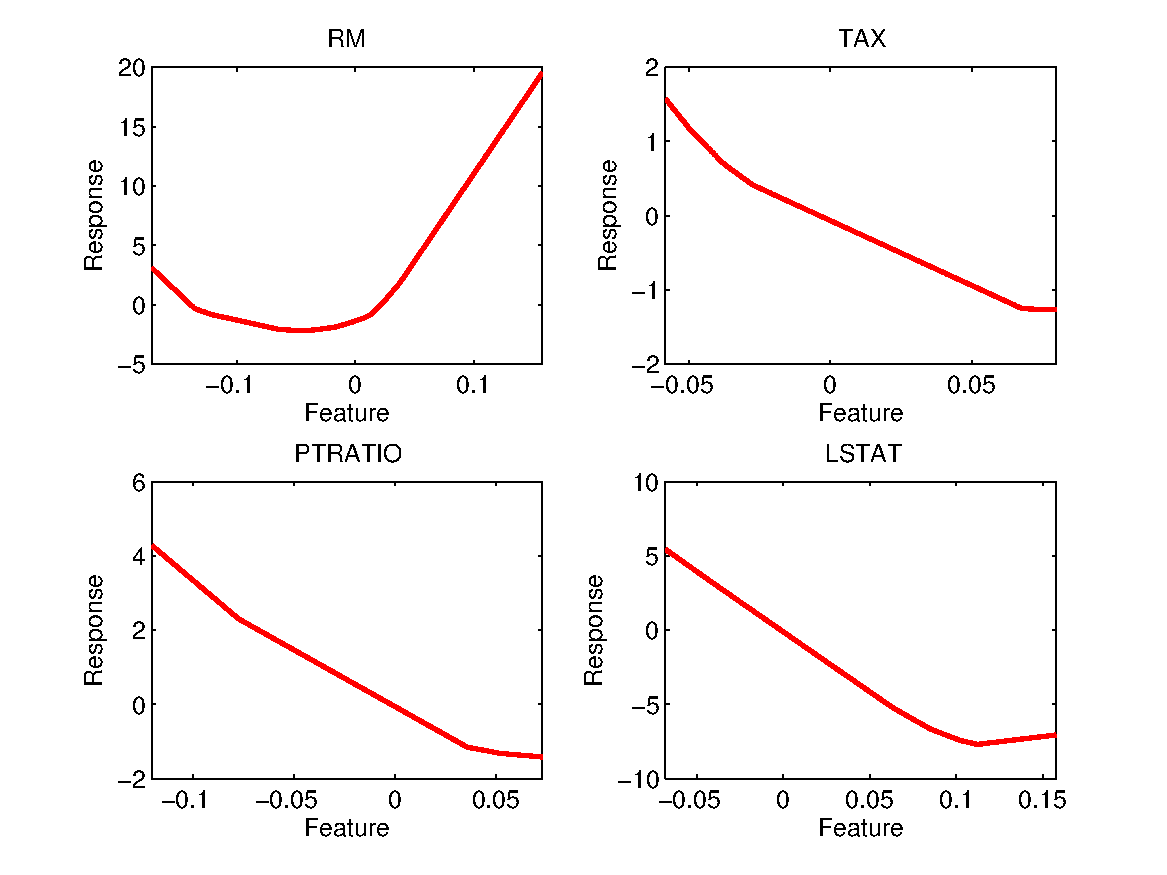
\includegraphics[width=\textwidth]{figs/Convex}
%                \caption{Inferred additive convex functions by SCAM.}
%                \label{Convex}
%        \end{subfigure}
%        \caption{Results on Boston housing data.}\label{Boston}
%\end{figure}


\begin{figure*}[!t]
\begin{center}
\begin{tabular}{cccc}
\hskip-10pt
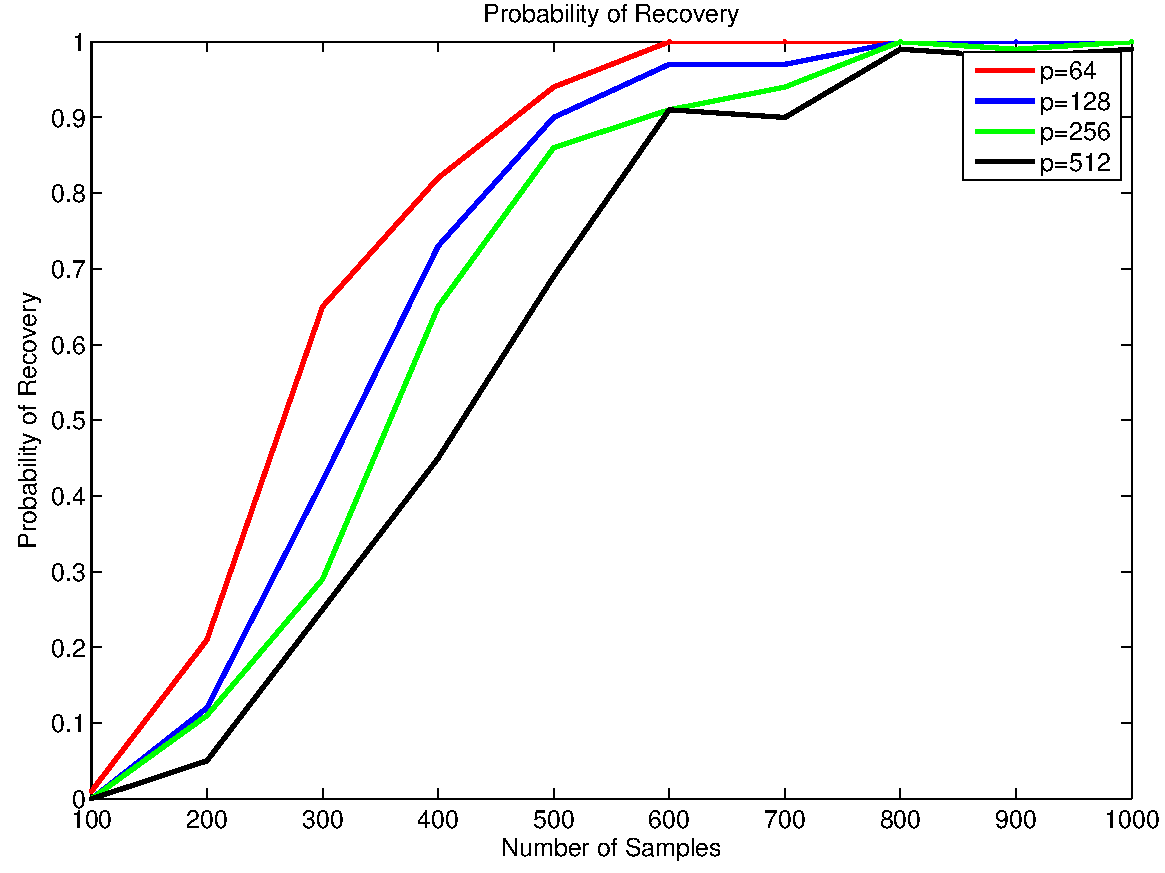
\includegraphics[width=.26\textwidth]{figs/Curve1} &
\hskip-10pt
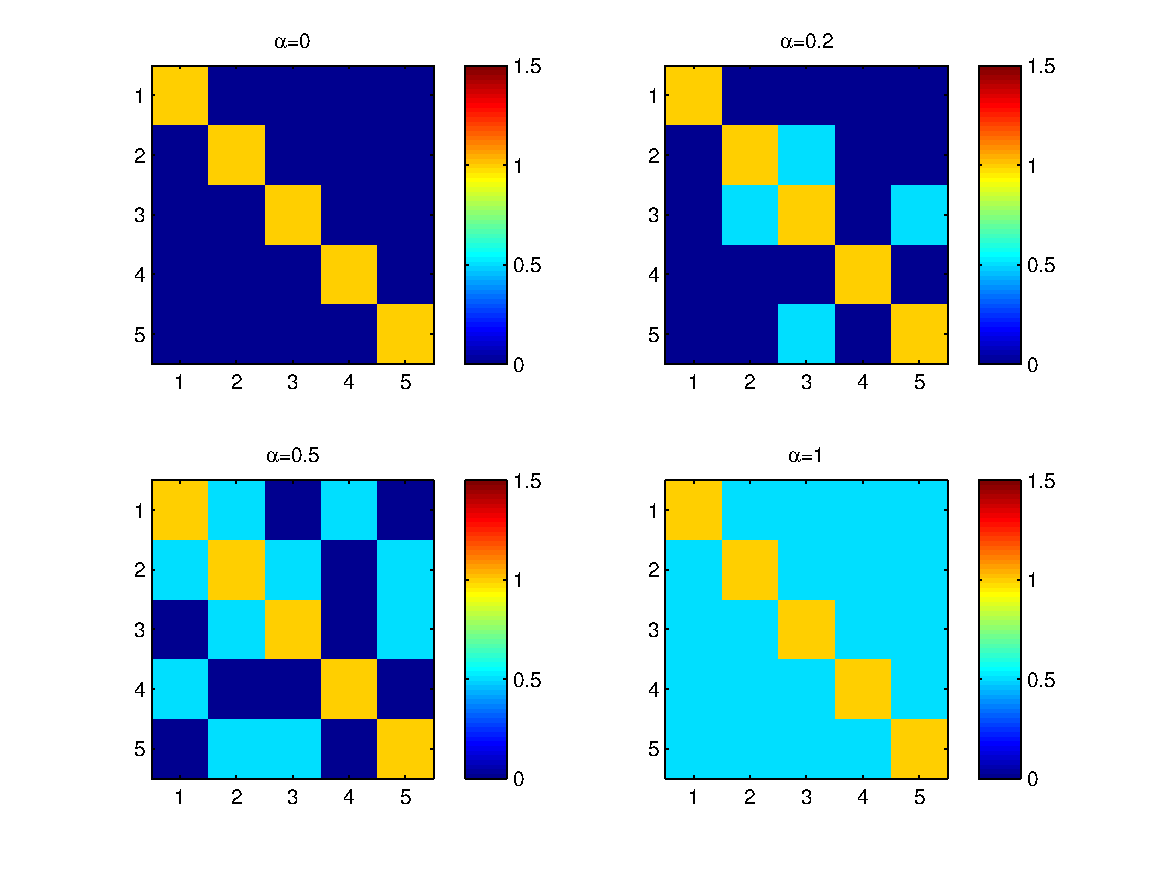
\includegraphics[width=.26\textwidth]{figs/Q} &
\hskip-10pt
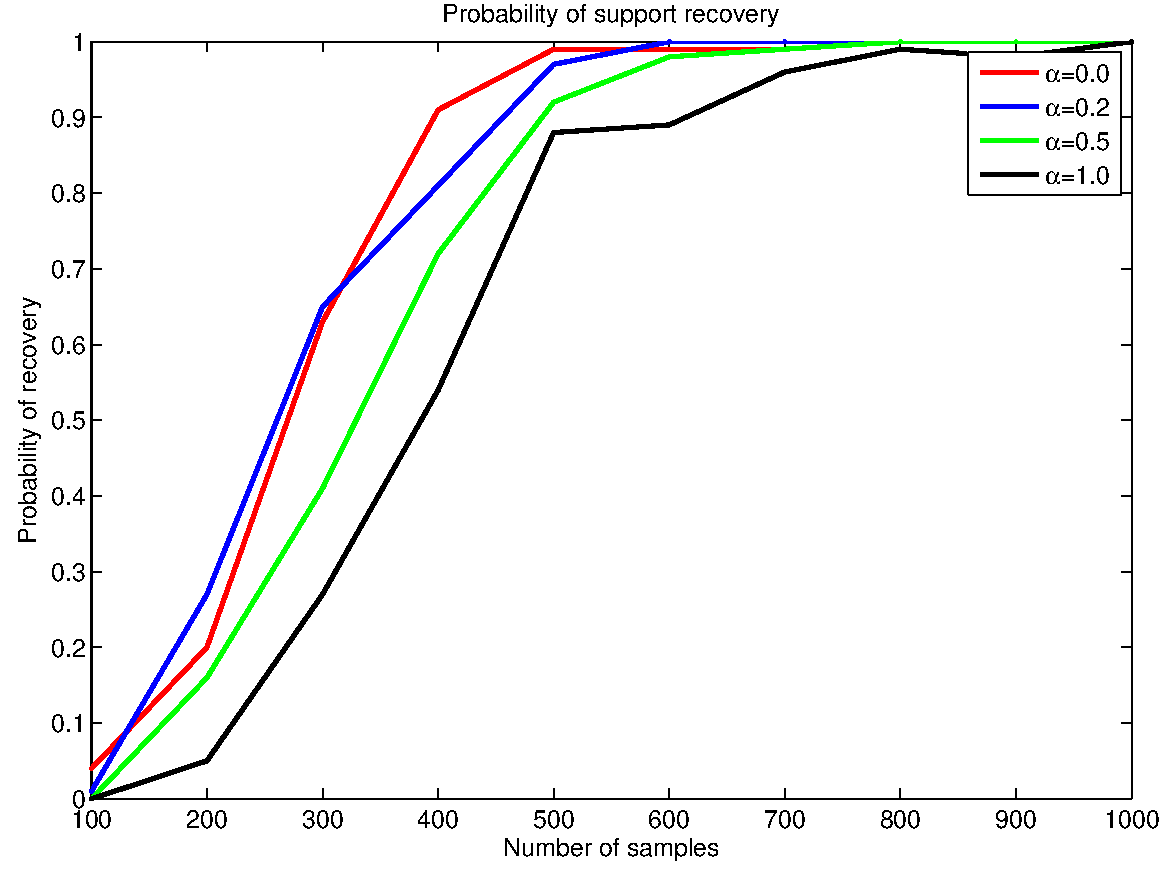
\includegraphics[width=.26\textwidth]{figs/Curve2} &
\hskip-10pt
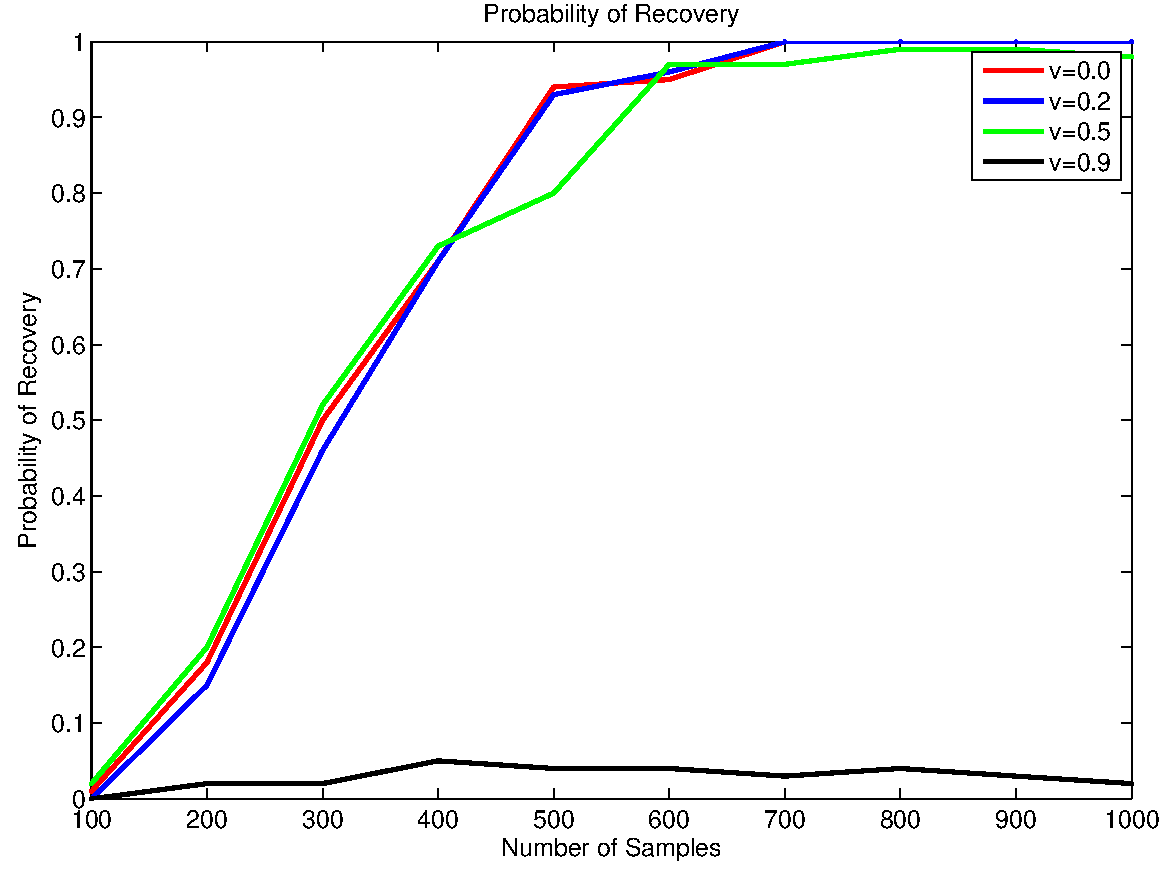
\includegraphics[width=.26\textwidth]{figs/Curve4}  \\
\hskip-10pt (a) additive model & 
\hskip-10pt (b) four $\Q$ matrices &
\hskip-10pt (c) non-additive models & 
\hskip-10pt (d) correlated design
\end{tabular}
\end{center}
\caption{Support recovery results where the additive assumption is
  correct (a), incorrect (b), (c), and with correlated design (d).}\label{Support}
\vskip10pt

\begin{center}
\begin{tabular}{ccc}
\hskip-10pt
  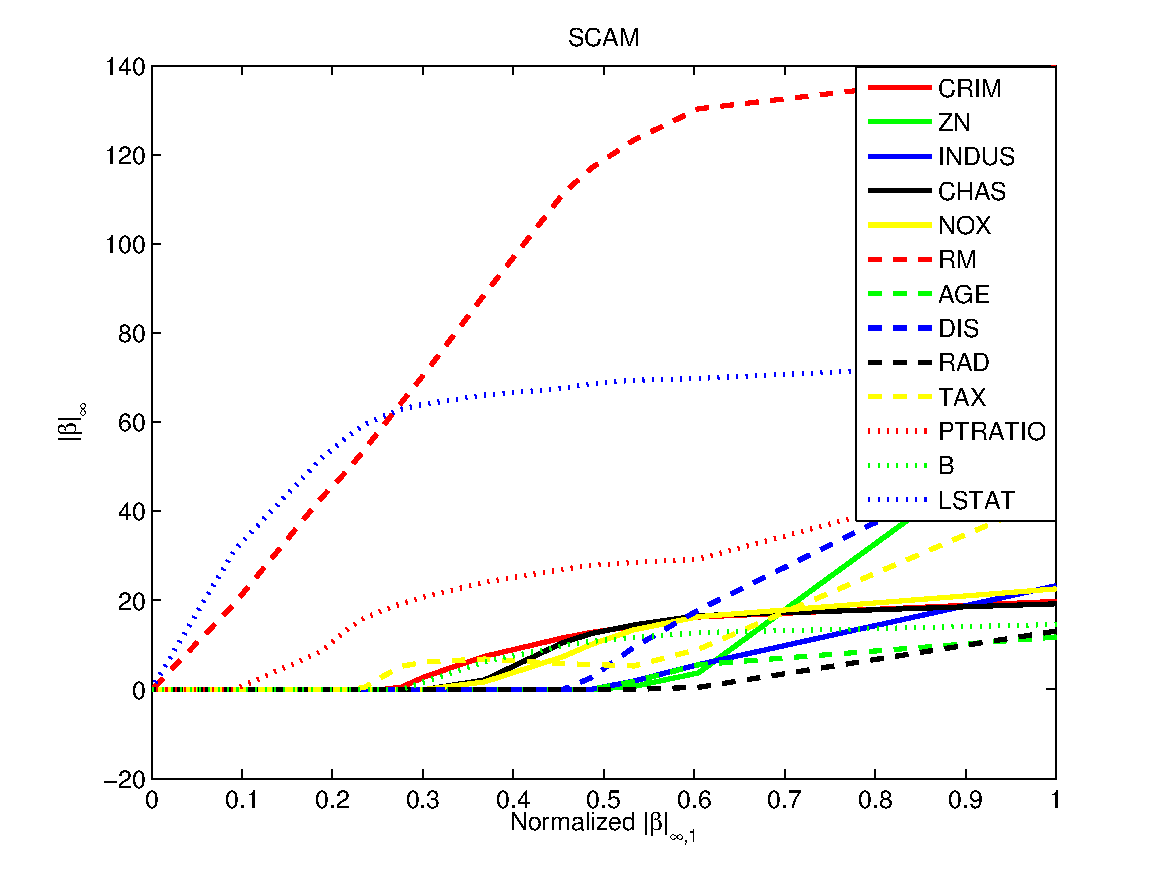
\includegraphics[width=.35\textwidth]{figs/Additive} &
\hskip-25pt
  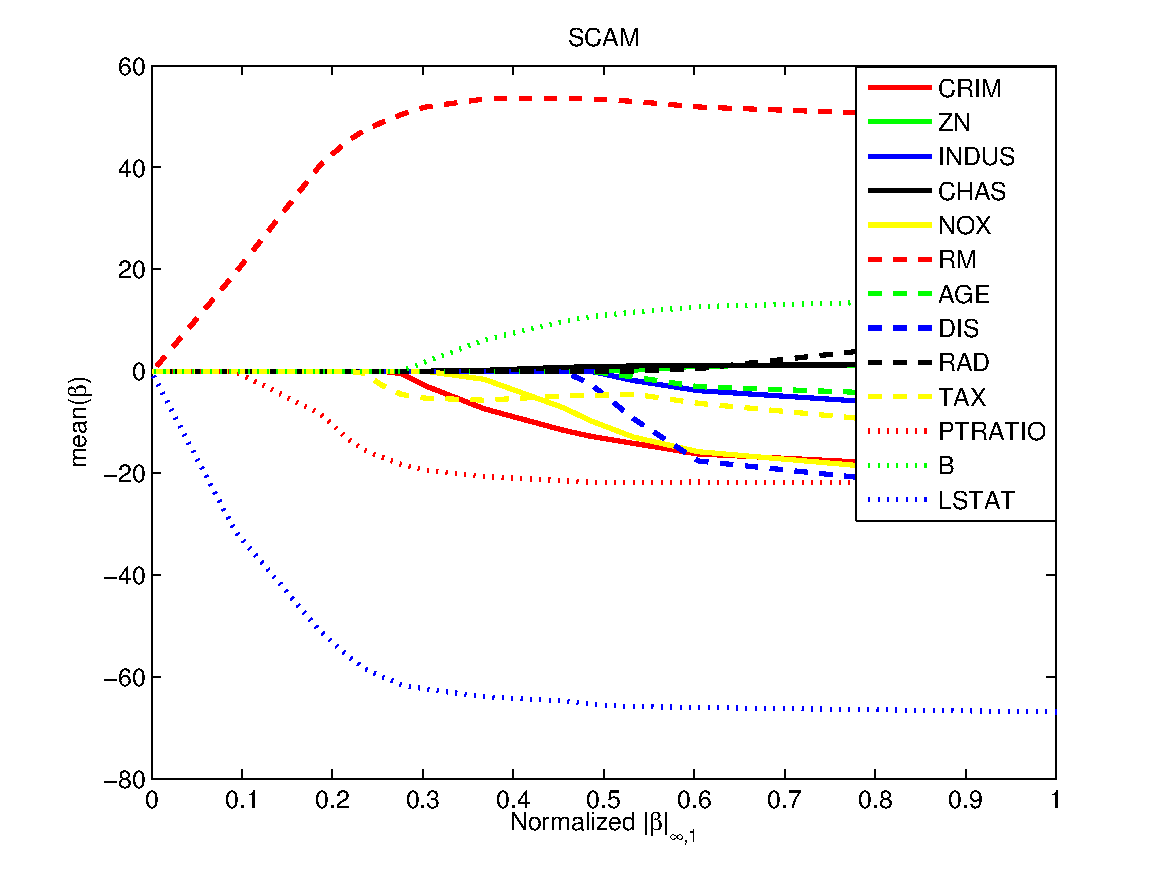
\includegraphics[width=.35\textwidth]{figs/Additive1} &
\hskip-25pt
  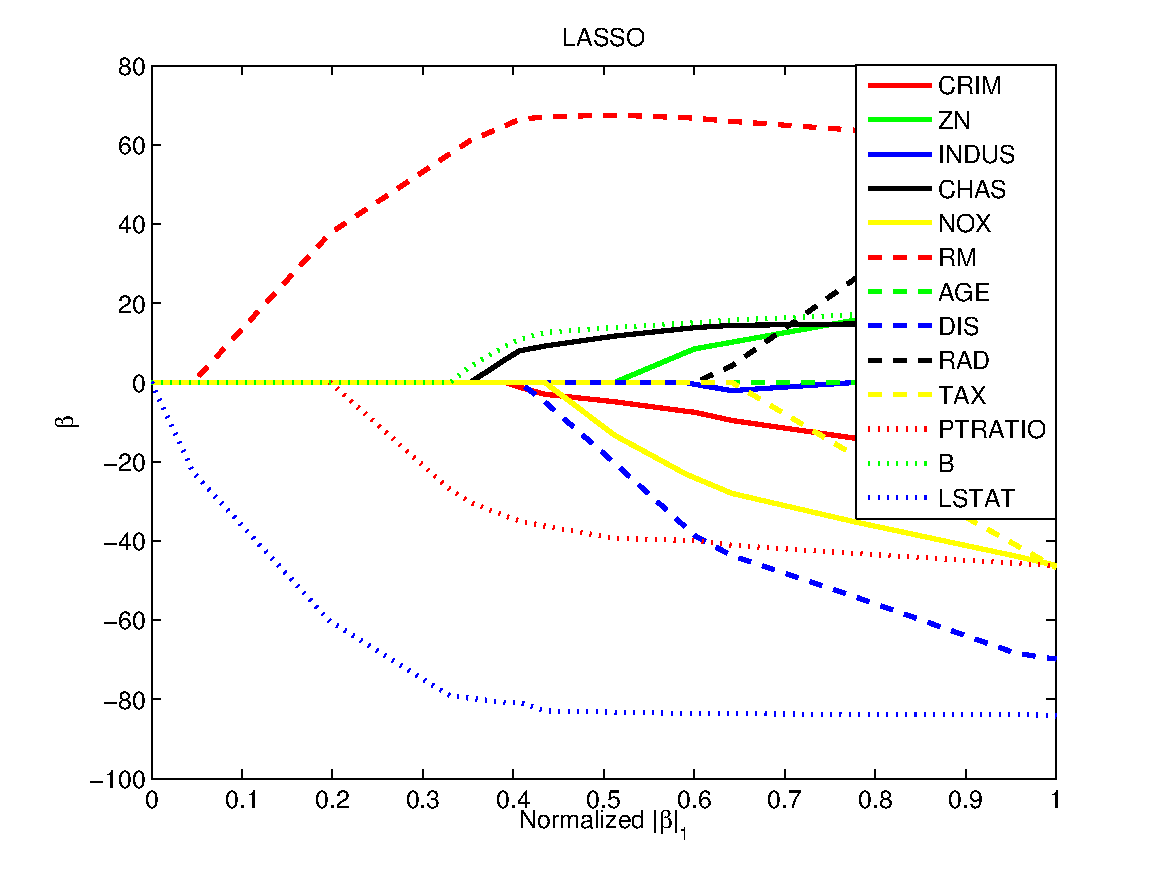
\includegraphics[width=.35\textwidth]{figs/LASSO} 
\\
\hskip-10pt 
SCAM $\|\beta_k\|_\infty$ paths & 
\hskip-25pt 
SCAM $\text{mean}(\beta_k)$ paths &
\hskip-25pt
LASSO $\beta_k$ paths
\end{tabular}
\begin{tabular}{cc}
  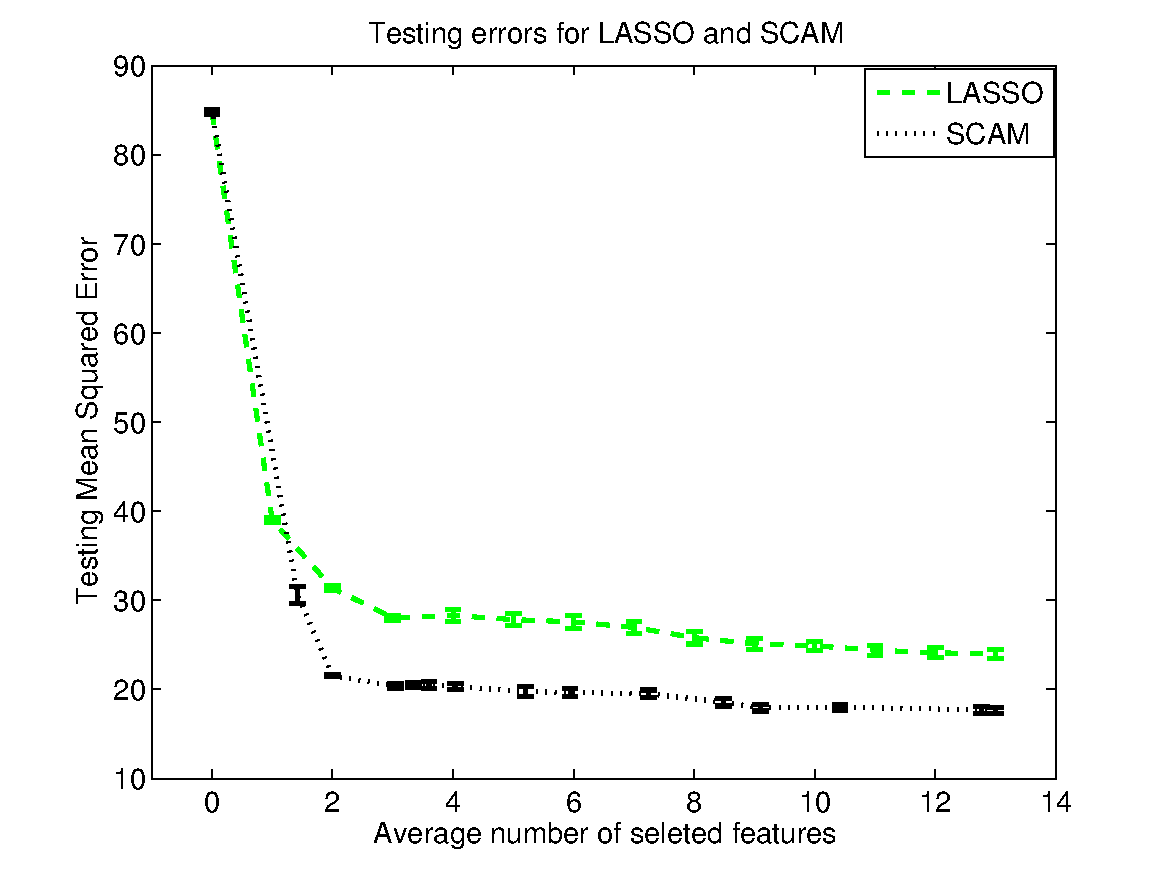
\includegraphics[width=.37\textwidth]{figs/MSE} &
  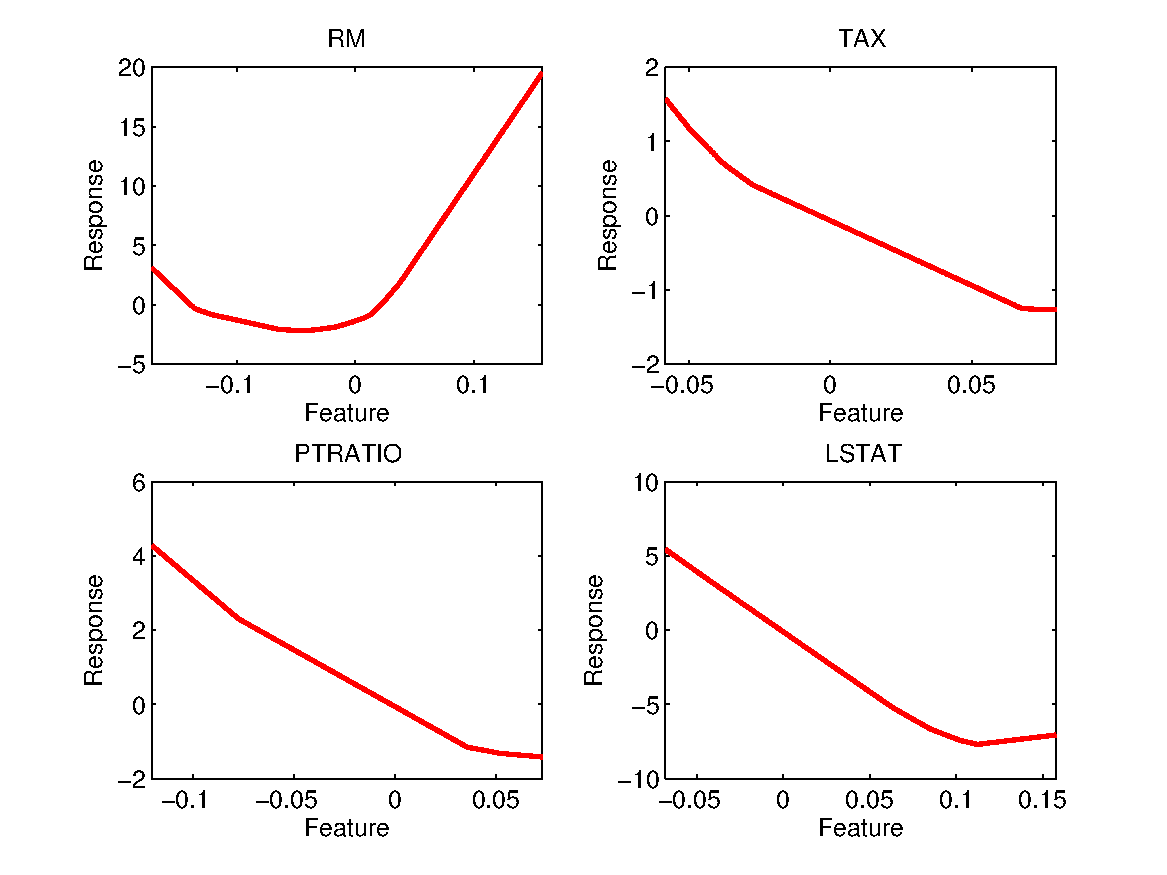
\includegraphics[width=.43\textwidth]{figs/Convex}
\\
predictive MSE & inferred functions from SCAM
\end{tabular}
\end{center}
\caption{Results on Boston housing data, showing regularization paths,
 MSE and fitted functions.}\label{Boston}
\end{figure*}


% DO NOT CHANGE; RefTex variables -minx
 
%%% Local Variables: ***
%%% mode:latex ***
%%% TeX-master: "paper.tex" ***
%%% End: ***

